% Created 2017-01-20 Fri 17:00
\documentclass[11pt]{article}
\usepackage[utf8]{inputenc}
\usepackage{lmodern}
\usepackage[T1]{fontenc}
\usepackage{fixltx2e}
\usepackage{graphicx}
\usepackage{longtable}
\usepackage{float}
\usepackage{wrapfig}
\usepackage{rotating}
\usepackage[normalem]{ulem}
\usepackage{amsmath}
\usepackage{textcomp}
\usepackage{marvosym}
\usepackage{wasysym}
\usepackage{amssymb}
\usepackage{amsmath}
\usepackage[version=3]{mhchem}
\usepackage[numbers,super,sort&compress]{natbib}
\usepackage{natmove}
\usepackage{url}
\usepackage{minted}
\usepackage{underscore}
\usepackage[linktocpage,pdfstartview=FitH,colorlinks,
linkcolor=blue,anchorcolor=blue,
citecolor=blue,filecolor=blue,menucolor=blue,urlcolor=blue]{hyperref}
\usepackage{attachfile}
\usepackage[top=1in, bottom=1.in, left=1in, right=1in]{geometry}
\author{Zhongnan Xu}
\date{2013-02-05 Tue}
\title{Tutorial for analyzing jobs using the DataExplorer}
\begin{document}

\maketitle
\tableofcontents

\section{Introduction}
\label{sec:orgheadline1}
The purpose of this is to work through some examples in using the DataExplorer to analyze optimization runs done by StructOpt. The example calculations we will be working with are held in the \textbf{job\(_{\text{manager}}_{\text{examples}}\)} folder. These jobs were submitted by the \texttt{JobManager} wrapper. All examples were of the optimization of a Au55 nanocluster.

\section{Initialization}
\label{sec:orgheadline2}
The initialization of the DataExplorer is done by specifying the \textbf{log\{time\}} directory where the calculation has been performed. If the directory name is known, initialization is simple. In contrast, if the user submitted the job using the \textbf{JobManager}, the directory which holds the \textbf{log\{time\}} directory can be used to locate a specific \textbf{logfr\{time\}} based on the order of which it was run.

\begin{minted}[frame=lines,fontsize=\scriptsize,linenos]{python}
from structopt.utilities.job_manager import JobManager
from structopt.utilities.data_explorer.core import DataExplorer

# Initialization if the logdir is known
logdir = 'job_manager_examples/Au55-example/logs20170120035711'
DE = DataExplorer(logdir)

# Initialization through the JobManager
calcdir = 'job_manager_examples/Au55-example'
job = JobManager(calcdir)
DE = job.get_data_explorer()
\end{minted}

\section{Analysis}
\label{sec:orgheadline7}
The scripts below are examples of how to read data out of calculations.

\subsection{Fitnesses}
\label{sec:orgheadline4}
\subsubsection{Long example}
\label{sec:orgheadline3}
The example below shows how one reads the fitness of the most fit individual in each generation. This first script is a long example that shows the structure of the DataExplorer once it is loaded. 

\begin{minted}[frame=lines,fontsize=\scriptsize,linenos]{python}
import numpy as np
import matplotlib.pyplot as plt
from structopt.utilities.job_manager import JobManager

# Initialization through the JobManager
calcdir = 'job_manager_examples/Au55-example'
job = JobManager(calcdir)
data = job.get_data_explorer()

average_fitnesses = []

for population in data:
    population_fitnesses = []
    for individual_id in population:
        individual = population[individual_id]
        population_fitnesses.append(individual.fitness)
    average_fitnesses.append(np.mean(population_fitnesses))

plt.figure(1, (4, 3))
plt.plot(range(len(average_fitnesses)), average_fitnesses, c='k')
plt.xlabel('Generation')
plt.ylabel('Fitness')
plt.tight_layout()
plt.savefig('images/average-fitness.png', dpi=300)
\end{minted}

\begin{figure}[htb]
\centering
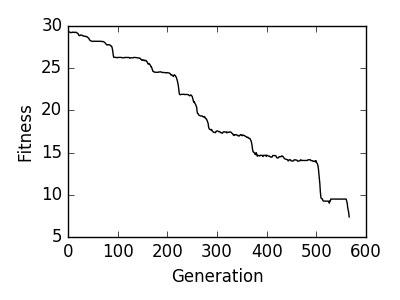
\includegraphics[width=.9\linewidth]{./images/average-fitness.png}
\caption{The evolution of the average fitness (total energy) of a Au55 nanoparticle}
\end{figure}

The \textbf{DataExplorer} object functions like a list of populations, so with index \emph{i} returns a \textbf{Population} object. The \textbf{Population} object functions like an dictionary, where the \textbf{id} of each individual is each key of the \textbf{Population}, and the value is an \textbf{Individual} object. When loaded through the \textbf{DataExplorer}, the \textbf{Individual} comes preloaded with a number of properties that provide information of it.

\subsection{Genealogy}
\label{sec:orgheadline5}
\subsection{Structures}
\label{sec:orgheadline6}
\end{document}